%%%%%%%%%%%%%%%%%%%%%%%%%%%%%%%%%%%%%%%%%%%%%%%%%%%%%%%%%%%%%%%%%%%%%%%%%%%%%%%
%% Resource-Normalized Scaling Laws for Byzantine Consensus
%% Peniak B.O., Liubinskiy B.B.
%%
%% COMPILE WITH pdflatex (T2A fontenc + babel). NOT xelatex / lualatex.
%%   pdflatex paper3 && pdflatex paper3
%% Bibliography is a manual `thebibliography' environment: NO bibtex / biblatex.
%%%%%%%%%%%%%%%%%%%%%%%%%%%%%%%%%%%%%%%%%%%%%%%%%%%%%%%%%%%%%%%%%%%%%%%%%%%%%%%

\documentclass[12pt]{article}
\usepackage{MMC}
\usepackage{graphicx}

%%%%%%%%%%%%%%%%%%%%%%%%%%%%%%%%%%%%%%%%%%%%%%%%%%%%%%%%%%%%%%%%%%%%%%%%%%%%%%%
%% macros.tex -- symbols of the model.
%% Rule: this file defines NOTATION only. Numeric results live in numbers.tex
%% and are generated by experiments/analysis/emit_numbers_tex.py.
%% Never hard-code a measured number in a section file.
%%%%%%%%%%%%%%%%%%%%%%%%%%%%%%%%%%%%%%%%%%%%%%%%%%%%%%%%%%%%%%%%%%%%%%%%%%%%%%%

%--------------------------------------------------------------- primary symbols
\newcommand{\n}{n}                  % validator count
\newcommand{\cc}{c}                 % client concurrency (number of senders)
\newcommand{\q}{q}                  % per-validator CPU quota (cores)
\newcommand{\w}{w}                  % detection window length (epochs)
\newcommand{\kf}{k}                 % number of faulty validators

%------------------------------------------------------------------ throughput
\newcommand{\TPS}{\mathrm{TPS}}
\newcommand{\TPSn}{\widetilde{\mathrm{TPS}}}   % resource-normalized throughput
\newcommand{\Tzero}{T_{0}}
\newcommand{\gfun}{g}                          % client-concurrency factor
\newcommand{\csat}{c^{\ast}}                   % saturation concurrency
\newcommand{\ahat}{\hat{\alpha}}               % single-factor (confounded) exponent
\newcommand{\bhat}{\hat{\beta}}
\newcommand{\ghat}{\hat{\gamma}}

%-------------------------------------------------------------------- detection
\newcommand{\Bhat}{\hat{B}}
\newcommand{\pd}{p_{d}}
\newcommand{\pf}{p_{f}}
\newcommand{\pmiss}{p_{\mathrm{miss}}}
\newcommand{\neff}{n_{\mathrm{eff}}}
\newcommand{\thr}{\tau}                        % override threshold

%----------------------------------------------------------------------- sizing
\newcommand{\Dpk}{D_{\mathrm{peak}}}
\newcommand{\epsp}{\varepsilon_{p}}
\newcommand{\epss}{\varepsilon_{s}}
\newcommand{\nmin}{n_{\min}}
\newcommand{\nmax}{n_{\max}}
\newcommand{\nopt}{n^{\ast}}
\newcommand{\Cost}{\mathrm{Cost}}
\newcommand{\Feas}{\mathcal{F}}
\newcommand{\kappaScale}{\kappa}          % production scale-up from RNM units

%------------------------------------------------------------------- statistics
% \Prob and \Var are pre-defined by babel-russian (mathsf forms); renew to the
% blackboard / roman forms used throughout the paper.
\newcommand{\E}{\mathbb{E}}
\renewcommand{\Prob}{\mathbb{P}}
\renewcommand{\Var}{\mathrm{Var}}
\newcommand{\Cov}{\mathrm{Cov}}
% Used as \zq_{1-\varepsilon}: bare symbol, not a one-argument macro.
\newcommand{\zq}{z}
\newcommand{\PI}{\mathrm{PI}}

%------------------------------------------------------------------- shorthands
\newcommand{\eqdef}{\mathrel{\mathop:}=}
\newcommand{\RNM}{RNM}
\newcommand{\ie}{i.\,e.}
\newcommand{\eg}{e.\,g.}

% Math-/tabular-safe TODO: MMC's \TODO uses \marginpar (fails in $...$ and
% floats). Arguments may contain `_` (e.g. n_max); \detokenize keeps them literal.
\renewcommand\TODO[1]{\mbox{\normalfont\color{red}\sffamily[TODO:\detokenize{#1}]}}

% babel-ukrainian 1.5a defines \Ukrainian as \selectlanguage{\ukrainian}
% (control sequence), but \ukrainian is never defined; russianb correctly uses
% the string form. Restore the working switch for MMC's \maketitleUkr.
\DeclareRobustCommand{\Ukrainian}{\selectlanguage{ukrainian}}
\providecommand{\English}{\selectlanguage{english}}

%%%%%%%%%%%%%%%%%%%%%%%%%%%%%%%%%%%%%%%%%%%%%%%%%%%%%%%%%%%%%%%%%%%%%%%%%%%%%%%
%% numbers.tex -- AUTO-GENERATED. DO NOT EDIT BY HAND.
%%
%% Regenerate with:
%%     python experiments/analysis/emit_numbers_tex.py \
%%            --in data/processed --out numbers.tex
%%
%% Any macro that still expands to a \TODO marker means the corresponding
%% quantity was not produced by the analysis pipeline.
%%%%%%%%%%%%%%%%%%%%%%%%%%%%%%%%%%%%%%%%%%%%%%%%%%%%%%%%%%%%%%%%%%%%%%%%%%%%%%%


%--- bi-factor calibration (X1, X3) ----------------------------------------------
\newcommand{\resBeta}{1.651}
\newcommand{\resBetaSE}{0.151}
\newcommand{\resGamma}{0.178}
\newcommand{\resGammaSE}{0.070}
\newcommand{\resCsat}{67.9}
\newcommand{\resTheta}{2.542}
\newcommand{\resTzero}{2016.5}
\newcommand{\resRsq}{0.727}
\newcommand{\resSigmaRes}{0.404}
\newcommand{\resCalibNobs}{48}

%--- confounding check (Theorem 1) -----------------------------------------------
\newcommand{\resLambda}{9.29}
\newcommand{\resAlphaHat}{-1.362}
\newcommand{\resAlphaPred}{-1.473}
\newcommand{\resAlphaHatLzero}{-1.548}
\newcommand{\resAlphaHatLone}{-1.362}
\newcommand{\resAlphaHatLtwo}{-0.661}

%--- model comparison holdout log-RMSE -------------------------------------------
\newcommand{\resRmseLinear}{1.329}
\newcommand{\resRmseSingle}{0.523}
\newcommand{\resRmseUsl}{0.637}
\newcommand{\resRmseOurs}{0.538}

%--- q-invariance (X2) -----------------------------------------------------------
\newcommand{\resBetaQlow}{1.550}
\newcommand{\resBetaQmid}{1.541}
\newcommand{\resBetaQhigh}{0.879}
\newcommand{\resQinvP}{0.002}
\newcommand{\resTpsQlowNfour}{55.5}
\newcommand{\resTpsQmidNfour}{68.6}
\newcommand{\resTpsQhighNfour}{70.0}
\newcommand{\resTpsMaxMeasured}{89}
\newcommand{\resTpsMaxN}{7}
\newcommand{\resTpsMaxC}{16}
\newcommand{\resTpsMaxQ}{0.25}
\newcommand{\resKappaQuotaRatio}{52}

%--- WAN degradation (X4) --------------------------------------------------------
\newcommand{\resBetaRttZero}{1.459}
\newcommand{\resBetaRttTwentyFive}{1.925}
\newcommand{\resBetaRttFifty}{0.252}
\newcommand{\resBetaRttHundred}{2.011}
\newcommand{\resBetaRttHigh}{2.708}
\newcommand{\resDeltaBetaRtt}{1.248}

%--- detector characterisation (X5) ----------------------------------------------
\newcommand{\resPd}{0.397}
\newcommand{\resPf}{0.376}
\newcommand{\resRho}{0.000}
\newcommand{\resAuc}{0.506}
\newcommand{\resYouden}{0.021}
\newcommand{\resDetRuns}{13}
\newcommand{\resDetMargin}{0.0107}
\newcommand{\resNminDet}{3329}

%--- prediction-interval coverage (X7) -------------------------------------------
\newcommand{\resCovNinety}{90.9\,\%}
\newcommand{\resCovNinetyFive}{95.5\,\%}
\newcommand{\resHoldoutRuns}{22}
\newcommand{\resCalibRuns}{45}
\newcommand{\resCalibMaxN}{9}
\newcommand{\resBetaCalibMaxN}{1.300}
\newcommand{\resBetaSmallN}{1.196}
\newcommand{\resBetaGapCalib}{2.3}
\newcommand{\resBetaGapSmallN}{3.0}
\newcommand{\resSmallNmax}{9}
\newcommand{\resBetaLocalA}{1.4}
\newcommand{\resBetaLocalB}{1.7}
\newcommand{\resBetaLocalC}{2.8}
\newcommand{\resKappaSmallN}{16.7}
\newcommand{\resCovHitsNinety}{20}
\newcommand{\resCovHitsNinetyFive}{21}
\newcommand{\resHoldoutN}{n \in \{11, 13, 16\}}

%--- sizing ablation (X8) --------------------------------------------------------
\newcommand{\resKappa}{13.0}
\newcommand{\resDemand}{2100}
\newcommand{\resKappaDoubled}{26.0}
\newcommand{\resKappaWan}{73.4}
\newcommand{\resKappaCalibC}{12.94}
\newcommand{\resCalibCmax}{16}
\newcommand{\resKappaMode}{auto_min_admissible}
\newcommand{\resCstar}{32}
\newcommand{\resNminCase}{4}
\newcommand{\resNmaxCase}{4}
\newcommand{\resNoptCase}{4}
\newcommand{\resDetectorThr}{0.90}
\newcommand{\resCostLinear}{4.00}
\newcommand{\resCostSingle}{1.50}
\newcommand{\resCostUsl}{1.50}
\newcommand{\resCostOurs}{1.00}

%--- campaign metadata -----------------------------------------------------------
\newcommand{\resNmaxMeasured}{16}
\newcommand{\resTotalRuns}{94}
\newcommand{\resCoreHours}{27.2}

% Line breaks after explicit hyphens make PDF text copy drop the hyphen.
\exhyphenpenalty=10000

%%%%%%%%%%%%%%%%%%%%%%%%%%%%%%%%%% METADATA (EN) %%%%%%%%%%%%%%%%%%%%%%%%%%%%%%%

\title[Resource-Normalized Scaling Laws for BFT Consensus]{Resource-Normalized
Scaling Laws for Byzantine Consensus: Chance-Constrained Validator-Set Sizing
from Commodity-CI Measurements}

\author[Peniak B.\,O.]{Peniak B.\,O., Liubinskiy B.\,B.}

\organization{%
\address{1}Lviv Polytechnic National University\\
12 S.~Bandera str., 79013, Lviv, Ukraine\\
\address{2}Institute of Applied Mathematics and Fundamental Sciences}

\email{bohdan.o.peniak@lpnu.ua}

\received{29 July 2026}

\abstract{%
Sizing a permissioned BFT validator set for \mbox{e-governance} trades
consensus throughput, which falls with~$\n$, against fault-detection power,
which rises with it. We propose resource-normalized measurement with a fixed
per-validator CPU quota; show that, in the unsaturated bi-factor model with
zero-mean noise, the single-factor OLS exponent tends to
$\gamma\lambda-\beta$ (an \mbox{omitted-variable} bias); and formulate
chance-constrained sizing with feasible set $[\nmin,\nmax]$. On four-core
public CI ($\n\le\resNmaxMeasured$) the exponent is stable at a fixed quota but
quota-dependent; the measured detector is near chance (AUC$\,=\,\resAuc$), so
the detection constraint is relaxed (not enforced) and throughput alone sets
the window. Coefficients are deployment-specific.
%
\keywords{Byzantine fault tolerance, consensus, scaling law, capacity planning,
chance-constrained optimization, e-governance}
\MSC{68M14, 68W20, 90C15, 62J02}
\udk{004.75:519.2}
}

%%%%%%%%%%%%%%%%%%%%%%%%%%%%%%%%% METADATA (UKR) %%%%%%%%%%%%%%%%%%%%%%%%%%%%%%%

\titleUkr[Ресурсно-нормовані закони масштабування BFT-консенсусу]{РЕСУРСНО-НОРМОВАНІ
ЗАКОНИ МАСШТАБУВАННЯ BFT-КОНСЕНСУСУ: ІМОВІРНІСНО-ОБМЕЖЕНЕ ВИЗНАЧЕННЯ РОЗМІРУ
МНОЖИНИ ВАЛІДАТОРІВ ЗА ВИМІРЮВАННЯМИ НА ТИПОВІЙ CI-ІНФРАСТРУКТУРІ}

\authorUkr[Пеняк Б.\,О.]{Пеняк Б.\,О., Любінський Б.\,Б.}

\organizationUkr{%
Національний університет <<Львівська політехніка>>\\
вул.~С.~Бандери, 12, 79013, Львів, Україна}

\abstractUkr{%
Визначення розміру BFT-множини валідаторів для електронного урядування
узгоджує пропускну здатність, що спадає з~$\n$, із силою виявлення відмов, що
з~$\n$ зростає. Запропоновано ресурсно-нормовані вимірювання з фіксованою
CPU-квотою валідатора; показано, що за ненасиченої двофакторної моделі з шумом
нульового середнього однофакторний показник МНК прямує до
$\gamma\lambda-\beta$ (зміщення через пропущену змінну); сформульовано задачу з
імовірнісними обмеженнями та вікном $[\nmin,\nmax]$. На чотириядерній
публічній CI ($\n\le\resNmaxMeasured$) показник стабільний за фіксованої квоти,
але залежить від її рівня; виміряний детектор близький до випадкового
(AUC$\,=\,\resAuc$), тож детекційне обмеження послаблено (не застосовується), і
вікно визначає лише пропускна здатність. Коефіцієнти специфічні для
розгортання.
%
\keywordsUkr{візантійська відмовостійкість, консенсус, закон масштабування,
планування потужності, оптимізація з імовірнісними обмеженнями, електронне
урядування}
\udkUkr{004.75:519.2}
}

%%%%%%%%%%%%%%%%%%%%%%%%%%%%%%%%%%%% BODY %%%%%%%%%%%%%%%%%%%%%%%%%%%%%%%%%%%%%%

\begin{document}

\maketitle

\section{Introduction}
\label{sec:intro}

Permissioned Byzantine Fault Tolerant (BFT) consensus underpins \mbox{e-governance}
systems --- voting, registries, digital identity --- and raises a concrete
procurement question: \emph{how many validators should the network have?}

The validator count~$\n$ pulls in opposite directions. Throughput argues for
small~$\n$: every validator executes every transaction, and PBFT-family
protocols exchange $O(\n^{2})$ messages per block. Detection reliability argues
for large~$\n$. This paper develops a reproducible engineering methodology that
combines the two under resource-normalized calibration.

A practical obstacle is that dedicated multi-host testbeds are often
unavailable at design time. Commodity CI runners are accessible and
reproducible, yet pack many validators onto few cores. Without normalization,
fitted exponents mix consensus cost with host contention and with the load
generator's concurrency schedule. Published single-factor fits
$\TPS(\n)\propto\n^{\alpha}$ then disagree in magnitude and sometimes in sign.
Our earlier studies, extrapolated to sixty validators, differ by roughly an
order of magnitude --- often read as protocol-specific behaviour. Within the
investigated setting we show that it can arise from measurement design alone.

\paragraph{Contributions.}
The central methodological contribution is resource-normalized measurement
(\RNM{}): fixed CPU quota~$\q$ per validator and $\TPSn=\TPS/\q$, calibrating
consensus cost separately from host contention; in the evaluated deployment it
stabilizes the exponent at a fixed quota, although the exponent still depends
on the quota level (Section~\ref{sec:exp}). Analytically, under the unsaturated
bi-factor model with zero-mean noise,
$\ahat_{m}\xrightarrow{\Prob}\gamma\lambda-\beta$ along a concurrency path
(Proposition~\ref{prop:identifiability}) --- the standard \mbox{omitted-variable}
bias~\cite{wooldridge2010}, used here to interpret measured single-factor
exponents and to show why an \RNM{} factorial design ($\lambda=0$) matters. We
also formulate chance-constrained sizing with feasible set $[\nmin,\nmax]$
(Proposition~\ref{prop:window}) and calibrate the workflow on public Besu/QBFT
commodity CI (Sections~\ref{sec:exp}--\ref{sec:case}). The
throughput--detection trade-off is formulated but not demonstrated: the
measured detector is near chance, the detection constraint is unsatisfiable
with it, and the window is set by throughput alone
(Section~\ref{sec:detection}). Coefficients are deployment-specific and
intended for recalibration; cross-client replication is out of scope.

\section{Related work}
\label{sec:related}

\emph{BFT protocols.}
Classical PBFT~\cite{castro1999} tolerates $f<\n/3$ at $O(\n^{2})$
messages~\cite{lamport1982,dwork1988}. Later designs ---
HotStuff~\cite{yin2019}, Tendermint~\cite{buchman2016},
Algorand~\cite{gilad2017}, HoneyBadgerBFT~\cite{miller2016} --- trade latency
and randomization; Vukoli\'{c}~\cite{vukolic2015} argues that no protocol
dominates. These lines of work fix the validator set; they do not size it under
joint throughput and detection requirements.

\emph{Benchmarks.}
Fabric~\cite{androulaki2018,thakkar2018}, BLOCKBENCH~\cite{dinh2017} and
BFT-SMaRt~\cite{sousa2018} report absolute throughput at chosen configurations.
They do not separate concurrency from validator count, nor state measurement
conditions under which fitted exponents would be expected to transfer.

\emph{Scalability characterization and tools.}
Amdahl~\cite{amdahl1967}, Gustafson~\cite{gustafson1988} and Gunther's
USL~\cite{gunther2007} fold concurrency and system size into one load variable
--- the confound that \RNM{} is designed to remove. Concentration
bounds~\cite{hoeffding1963,boucheron2013}, Kish's design
effect~\cite{kish1965}, delta-method intervals~\cite{seber2003}, the residual
bootstrap~\cite{efron1993}, \mbox{omitted-variable} bias in misspecified
regressions~\cite{wooldridge2010} and chance-constrained
programming~\cite{charnes1959,nemirovski2007} are standard instruments.

\emph{Prior work.}
Remote-voting analyses~\cite{springall2014,specter2020,park2021} place endpoint
and coercion threats out of scope. Our earlier
calibration~\cite{peniak2026a} and switching study~\cite{peniak2026b} left open
an identifiable consensus exponent and sizing with measured detector rates.

\section{Resource-normalized measurement and the bi-factor law}
\label{sec:model}

We introduce an isolation protocol, a bi-factor characterization, and an
identifiability result under stated assumptions.

\subsection{Resource-normalized measurement as an isolation tool}

If $\n$ validators share a host of $Q$ cores, each receives $Q/\n$ cores, so
measured throughput mixes algorithmic cost with a shrinking compute budget.
\RNM{} is designed to isolate those effects under controlled quotas.

\begin{Def}[Resource-normalized measurement]
\label{def:rnm}
A campaign follows the \emph{\RNM{} protocol} with quota~$\q$ if every validator
container receives the same CPU quota and memory limit independently of~$\n$,
with aggregate reservation $\n\q$ not exceeding host capacity. Normalized
throughput is
$\TPSn\eqdef\TPS/\q$.
\end{Def}

\begin{Assumption}[Separable compute budget]
\label{as:separable}
On the operating range of quotas in the campaign,
$\TPS(\n,\cc,\q)=\q\cdot\Phi(\n,\cc)\cdot(1+r)$ with $|r|\le C\q$ for a
constant~$C$ independent of~$(\n,\cc)$ there.
\end{Assumption}

\paragraph{Assumption check.}
Under Assumption~\ref{as:separable} and a power-law factor
$\Phi\propto\n^{-\beta}$, the OLS slope of $\log\TPSn$ on $\log\n$ at fixed
concurrency is independent of~$\q$: the relative remainder is absorbed by the
intercept. Section~\ref{sec:exp} tests this invariance across
$\q\in\{0.20,0.25,0.33\}$ and rejects it at $\q=0.33$: \RNM{} stabilizes
$\beta$ at a fixed quota rather than making it quota-free. The calibrated model
is reported at $\q=0.25$; outside that regime the coefficients must be re-fit.

\begin{Def}[Bi-factor scaling characterization]
\label{def:bifactor}
Under the \RNM{} protocol,
\begin{equation}
\TPS(\n,\cc)=\Tzero\cdot\gfun(\cc)\cdot\n^{-\beta},
\quad
\gfun(\cc)=\frac{\cc^{\gamma}}{1+(\cc/\csat)^{\theta}},
\label{eq:bifactor}
\end{equation}
with $\Tzero>0$, $\beta>0$, $\gamma\in(0,1]$, $\theta>\gamma$, $\csat>0$.
In the unsaturated regime $\cc\ll\csat$ this is log-linear:
$\log\TPS=\log\Tzero+\gamma\log\cc-\beta\log\n$.
\end{Def}

The form separates concurrency from validator-count scaling, reduces to a
power law for $\cc\ll\csat$, saturates at large~$\cc$, and contains the
classical single-factor fit as the case $\gamma=0$ (or $\lambda=0$ with
$\alpha=-\beta$).

\subsection{Identifiability}

Proposition~\ref{prop:identifiability} is the textbook \mbox{omitted-variable} bias of
regressing $\log\TPS$ on $\log\n$ while omitting $\log\cc$~\cite{wooldridge2010},
valid under the unsaturated bi-factor model and the stated path and noise
assumptions. Its value is interpretive: it shows how to read a measured
single-factor exponent under a stated concurrency path. Section~\ref{sec:exp}
checks consistency within the evaluated deployment only.

\begin{Proposition}[Identifiability of the consensus exponent]
\label{prop:identifiability}
Let observations follow the unsaturated bi-factor law with additive noise of
mean zero and finite variance, along a concurrency path
$\log\cc_{i}=\lambda\log\n_{i}+\mu+\eta_{i}$
($\E[\eta_{i}\mid\n_{i}]=0$). If the empirical second moment of
$x_{i}=\log\n_{i}$ converges to a positive limit, the OLS slope $\ahat_{m}$ of
$\log\TPS_{i}$ on $x_{i}$ alone satisfies
$\ahat_{m}\xrightarrow{\Prob}\gamma\lambda-\beta$.
In particular $\ahat>0\iff\lambda>\beta/\gamma$, and $\ahat=-\beta\iff\lambda=0$.
\end{Proposition}

\begin{Proof}
With $x_{i}=\log\n_{i}$, the path reduces the unsaturated law to
$\log\TPS_{i}=a+\alpha x_{i}+\varepsilon_{i}$, $\E[\varepsilon_{i}\mid x_{i}]=0$,
finite variance, and
$\alpha=\underbrace{-\beta}_{\text{protocol}}
+\underbrace{\gamma\lambda}_{\text{measurement}}$.
OLS consistency under the second-moment condition gives
$\ahat_{m}\xrightarrow{\Prob}\alpha$~\cite{wooldridge2010}; signs follow from
$\gamma>0$.
\end{Proof}

Under the stated model, only a factorial design ($\lambda=0$) makes the
single-factor slope a consistent estimate of~$-\beta$. For illustration,
hypothetical values $\gamma=0.8$, $\beta=0.5$ and $\lambda=1$ (not the fitted
ones) yield $\ahat=+0.3$, and extrapolating from $\n=5$ to $\n=60$ differs by a
factor $\approx7$, matching the order of the discrepancy
in~\cite{peniak2026a}.

\begin{Corollary}[Non-transferability of single-factor exponents]
\label{cor:sign}
Under the unsaturated bi-factor model, laboratories measuring along
$\lambda_{1}\ne\lambda_{2}$ obtain exponents differing by
$\gamma(\lambda_{1}-\lambda_{2})$. Without reporting~$\lambda$, published
single-factor exponents should not be treated as transferable protocol
properties across measurement designs.
\end{Corollary}

\paragraph{Implementation.}
On a factorial grid ($\lambda=0$) we estimate $(\log\Tzero,\gamma,\beta)$ by
OLS in log-space and $(\csat,\theta)$ by nonlinear least squares on the full
$\cc$-sweep (Section~\ref{sec:exp}).

\section{Prediction intervals, detection, and the sizing problem}
\label{sec:sizing}

The workflow combines a throughput chance constraint with an optional detection
constraint; any detector yielding measured $(\pd,\pf,\rho)$ plugs in.

\subsection{Definitions and assumptions}

\begin{Def}[Fault class and detector]
\label{def:faults}
A subset $B$ of size $\kf$ is \emph{faulty} if each member fails a proposal
round independently with probability~$\pd$, while honest validators fail with
probability $\pf<\pd$ (omission class; equivocation excluded). The detector
flags validator~$i$ when its failure rate over $\w$ rounds exceeds
$\thr\in(\pf,\pd)$; detection succeeds when at least one member of~$B$ is
flagged.
\end{Def}

\begin{Assumption}[Exchangeable correlation]
\label{as:rho}
Participation indicators in~$B$ are exchangeable with pairwise correlation
$\rho\in[0,1)$, so the mean carries design effect $1+(\kf-1)\rho$ in the sense
of Kish~\cite{kish1965}.
\end{Assumption}

\subsection{Prediction intervals and detection bound}
\label{sec:detection}

With regressor $\mathbf{z}=(1,\log\cc,-\log\n)^{\!\top}$ and
$\hat\vartheta=(\log\Tzero,\gamma,\beta)^{\!\top}$, the delta
method~\cite{seber2003} gives predictive variance
$\hat{V}=\mathbf{z}^{\!\top}\widehat{\Cov}(\hat\vartheta)\mathbf{z}+\hat\sigma^{2}$.
An approximate $(1-\epsp)$ prediction interval for $\TPS(\n,\cc)$ is then
$\exp\{\log\widehat{\TPS}\mp\zq_{1-\epsp/2}\hat{V}^{1/2}\}$;\label{st:pi}
the one-sided lower endpoint $\underline{\TPS}_{1-\epsp}$ uses $\zq_{1-\epsp}$.
A residual bootstrap~\cite{efron1993} supplies empirical quantiles when residual
normality is doubtful. Coverage is checked on held-out validator counts within
the calibrated range (Section~\ref{sec:exp}).

With $\kf=\lceil\phi\n\rceil$, a design-effect heuristic yields the approximate
miss probability\label{st:rho}
\begin{equation}
\pmiss(\n,\w)\lesssim\exp\!\Bigl\{-\frac{2\w\kf(\pd-\thr)^{2}}{1+(\kf-1)\rho}\Bigr\},
\label{eq:pmiss}
\end{equation}
which is nonincreasing in $\n$ and $\w$. The cut $\pmiss\le\epss$ gives
\begin{equation}
\nmin=\left\lceil
\frac{1+(\kf-1)\rho}{\phi}\cdot
\frac{\log(1/\epss)}{2\w(\pd-\thr)^{2}}\right\rceil .
\label{eq:nmin}
\end{equation}
Expression~\eqref{eq:pmiss} is an engineering approximation adapting
Hoeffding~\cite{hoeffding1963} via Kish~\cite{kish1965}
($\neff=\kf\w/(1+(\kf-1)\rho)$), not a new exact bound.

\paragraph{Measured detector.}
X5 reports per-validator flag rates at the Youden-optimal participation
threshold~$0.90$: $\hat p_{d}=\resPd$ for faulty and $\hat p_{f}=\resPf$ for
honest validators ($J=\resYouden$). Plugging them into~\eqref{eq:nmin} with
$\thr$ at their midpoint, $\rho=0$, $\phi=0.2$, $\w=30$ and $\epss=0.01$ gives
$\nmin\approx\resNminDet$, far above any throughput-feasible~$\n$. With this
detector the detection constraint is unsatisfiable, so the formal feasible set
is empty; we relax it (do not enforce it): reported windows use $\nmin=4$
($3f+1$ with $f=1$) and are set by throughput alone. The two-constraint program applies to detectors with $J$
bounded away from zero; its trade-off is not demonstrated here.

\subsection{The sizing program}

\begin{Problem}[Validator-set sizing]
\label{prob:sizing}
Given peak demand $\Dpk$, levels $\epsp,\epss$, window~$\w$, faulty fraction
$\phi$, production scale-up $\kappaScale>0$ from \RNM{} units to absolute
throughput, and nondecreasing $\Cost(\n)$, minimize $\Cost(\n)$ subject to
$\Prob[\kappaScale\cdot\TPSn(\n,\cc^{\star})\ge\Dpk]\ge1-\epsp$ and
$\pmiss(\n,\w)\le\epss$, where $\cc^{\star}=\arg\max\gfun$. When $\kappaScale$
is free, take the smallest value that meets the throughput constraint at
$\n=4$.
\end{Problem}

The chance constraint is equivalent, via the prediction interval above, to
\begin{equation}
h(\n)\eqdef\log(\kappaScale\,\Tzero\,\gfun(\cc^{\star})/\Dpk)
-\beta\log\n-\zq_{1-\epsp}\hat{V}^{1/2}(\n,\cc^{\star})\ge0.
\label{eq:h}
\end{equation}
On the model-based extrapolation range ($\n\ge\resNmaxMeasured$) the fitted
covariance makes $\hat{V}$ nondecreasing in $\log\n$, so with
$\beta>0$ the map $h$ is strictly decreasing there; on the measured grid we
evaluate~$h$ directly.

\begin{Proposition}[Feasibility window]
\label{prop:window}
Whenever $h$ is strictly decreasing and the approximate detection cut
\eqref{eq:nmin} is used, the feasible set is
$\{\n:\nmin\le\n\le\nmax\}$ with $\nmin$ from~\eqref{eq:nmin} and
$\nmax=\lfloor\sup\{\n:h(\n)\ge0\}\rfloor$. If nonempty and $\Cost$ is
nondecreasing then $\nopt=\nmin$.
\end{Proposition}

\begin{Proof}
Detection holds on $\{\n\ge\nmin\}$ and throughput on $\{\n\le\nmax\}$, hence an
interval; monotone cost selects the left endpoint.
\end{Proof}

\begin{Corollary}[Empty feasible set]
\label{cor:infeasible}
If $\nmin>\nmax$, no validator count satisfies both requirements under the
stated constraints: the architecture must change, not merely the provisioning.
\end{Corollary}

Protocol-efficient sizes are $\n=3f+1$; other counts appear on the measurement
grid, but a procurement decision intersects the window with $\{3f+1\}$. The
window is the intersection of two monotone constraints
\cite{charnes1959,nemirovski2007}. Within the proposed methodology it converts
a calibrated model into a reproducible sizing workflow for the evaluated
deployment class.

\section{Experimental campaign on commodity CI}
\label{sec:exp}

\subsection{Setup and design}

The campaign runs in a public continuous-integration workflow on a four-core,
16~GB hosted runner. Constrained CI is the intended calibration setting:
accessible, reproducible, and usable when dedicated clusters are unavailable.
Each job provisions a Hyperledger Besu~\cite{besu} QBFT network of~$\n$
validators under the \RNM{} protocol (Definition~\ref{def:rnm}). A closed-loop
generator drives~$\cc$ concurrent submitters and records steady-state committed
throughput after warm-up. Faults are injected with kernel traffic control
(omission and duplication; not equivocation).

\textbf{X1}/\textbf{X3} calibrate $(\beta,\gamma)$ on a factorial grid;
\textbf{X2} checks the quota regime; \textbf{X3b} re-samples along
concurrency paths; \textbf{X4} varies emulated RTT; \textbf{X5} reports
detector rates; \textbf{X7}/\textbf{X8} check prediction-interval coverage and
sizing ablation. Cross-client replication (\textbf{X9}/GoQuorum) is out of
scope. In total $\resTotalRuns$ successful records,
$\approx\resCoreHours$ core-hours, $\n_{\max}=\resNmaxMeasured$.

\paragraph{Reproducibility.}
All experiments are reproducible from the public CI workflow and archived
artefacts at \url{https://github.com/bpenyak/Resource_Normalized_Scaling_Laws_for_Byzantine_Consensus}.

\subsection{Results}

\emph{X1/X3 --- bi-factor calibration.}
Joint OLS on the $\resCalibNobs$ unsaturated fault-free runs at the reference
quota ($\n\in\{4,\dots,16\}$, $\cc\in\{1,\dots,16\}$) yields
$\beta=\resBeta\pm\resBetaSE$ and $\gamma=\resGamma\pm\resGammaSE$
($R^{2}=\resRsq$; Table~\ref{tab:results}) at fixed concurrency and
$\q=0.25$, using all counts including the hold-out ones. A constant $\beta$
averages a steepening slope: locally $\approx\resBetaLocalA$,
$\resBetaLocalB$, $\resBetaLocalC$ over $\n=4$--$7$, $7$--$13$, $13$--$16$ at
$\cc=16$, and refits on $\n\le\resSmallNmax$ give $\resBetaCalibMaxN$ (pooled
quotas) and $\resBetaSmallN$ (reference quota), $\resBetaGapCalib$ and
$\resBetaGapSmallN$ standard errors lower. We attribute this to host
contention as $\n\q$ approaches the four host cores shared with the load
generator ($\n\q=4$ at $\n=16$): \RNM{} removes contention only while $\n\q$
stays below the host cores. The headline $\beta$ is conservative for $\nmax$
but optimistic for $\kappaScale$ ($\resKappa$ vs.\ $\resKappaSmallN$ under the
$\n\le\resSmallNmax$ refit); the window $[4,4]$ holds under either fit by
construction.

\emph{X3b --- path check of Proposition~\ref{prop:identifiability}.}
A single-factor fit along $\lambda=1$ gives $\ahat=\resAlphaHat$ against
$\gamma\lambda-\beta=\resAlphaPred$.
Figure~\ref{fig:confounding} shows measured exponents tracking
$\gamma\lambda-\beta$ --- consistency with the analytical prediction, not
universal validity of the bi-factor form. The predicted sign change
($\lambda\approx\resLambda$) lies outside the tested $\lambda\in\{0,1,2\}$, so
the check tests the size of the shift, not the sign flip.

\begin{figure}[!t]
\centering
\begin{minipage}[t]{0.32\textwidth}
\centering
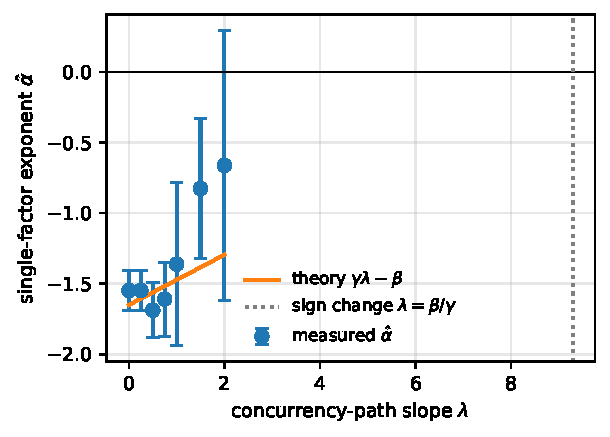
\includegraphics[width=\textwidth]{figures/fig_confounding}
\caption{Measured $\ahat$ (points) vs.\ analytical $\gamma\lambda-\beta$
(line) (Proposition~\ref{prop:identifiability}); predicted sign change at
$\lambda=\resLambda$, outside the tested paths}
\label{fig:confounding}
\end{minipage}\hfill
\begin{minipage}[t]{0.31\textwidth}
\centering
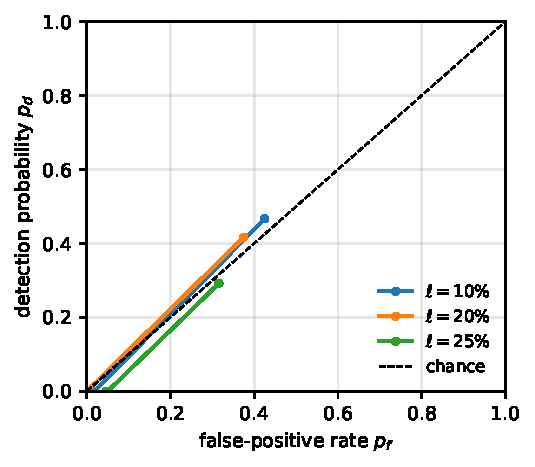
\includegraphics[width=\textwidth]{figures/fig_roc}
\caption{Measured detector ROC (AUC$\,=\,\resAuc$, near chance); the
detection constraint is unsatisfiable with it}
\label{fig:roc}
\end{minipage}\hfill
\begin{minipage}[t]{0.32\textwidth}
\centering
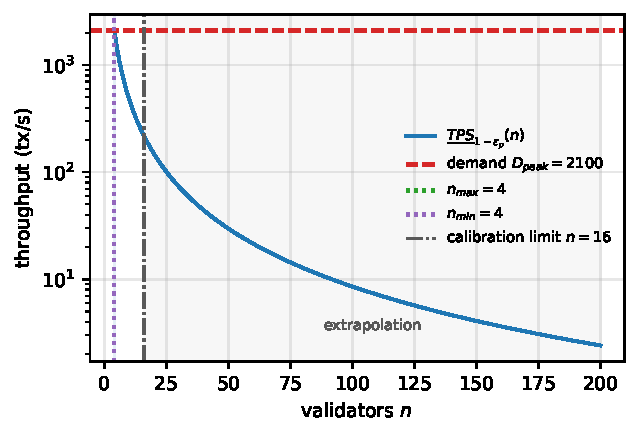
\includegraphics[width=\textwidth]{figures/fig_window}
\caption{Scenario~A: lower PI throughput vs.\ $\n$ at
$\kappaScale=\resKappa$; window $[\resNminCase,\resNmaxCase]$; dash-dotted:
calibration limit $\n=\resNmaxMeasured$}
\label{fig:window}
\end{minipage}
\end{figure}

\emph{X2 --- quota regime.}
X2 measures $\n\in\{4,7,13\}$ at $\cc=16$. The partial $F$-test for
quota\,$\times\log\n$ interaction rejects a common slope ($p=\resQinvP$):
$\beta$ is $\resBetaQlow$ and $\resBetaQmid$ at $\q=0.20,0.25$ but
$\resBetaQhigh$ at $\q=0.33$. In the $\q=0.33$ cells, throughput at $\n=4$ no
longer grows with the quota ($\resTpsQlowNfour$, $\resTpsQmidNfour$,
$\resTpsQhighNfour$~TPS), suggesting a non-CPU ceiling that breaks
Assumption~\ref{as:separable}, and at $\n=13$ the reservation of $\approx4.3$
cores exceeds the host, outside Definition~\ref{def:rnm}. \RNM{} thus
stabilizes $\beta$ at a fixed quota in the CPU-bound regime but does not make
it quota-free; coefficients are reported at $\q=0.25$.

\emph{X4 --- latency.}
On its own grid ($\n\in\{7,13\}$, $\cc=16$, $\q=0.25$), X4 gives
$\beta=\resBetaRttZero$ at $0$~ms and $\resBetaRttHigh$ at $200$~ms RTT
($\Delta\beta=\resDeltaBetaRtt$). The baseline is a two-point slope from four
runs and agrees with the joint fit $\beta=\resBeta$ within $1.3$ standard
errors; intermediate RTTs are non-monotone (Table~\ref{tab:results}), so X4
indicates the direction and rough size of the WAN penalty, not a latency law.

\emph{X5 --- detector.}
Over $\resDetRuns$ fault-injection runs the pooled ROC has
AUC$\,=\,\resAuc$ (Figure~\ref{fig:roc}, near chance); $\rho$ is not
identifiable from these runs and is set to~$0$. With these rates the detection
constraint is unsatisfiable and is relaxed, not enforced
(Section~\ref{sec:detection}).

\begin{table}[!t]
\centering
\caption{Calibrated parameters, quota check, detector, and coverage
(evaluated deployment)}
\label{tab:results}
\scriptsize
\begin{tabular}{lll}
\headline
Quantity & Estimate & Note \\
\headline
$\Tzero$; $\beta$; $\gamma$ &
  $\resTzero$; $\resBeta\pm\resBetaSE$; $\resGamma\pm\resGammaSE$ &
  bi-factor \\
$\csat$, $\theta$; $\hat\sigma$ & $\resCsat$, $\resTheta$; $\resSigmaRes$ &
  saturation / residual \\
$\ahat$ at $\lambda=0,1,2$ &
  $\resAlphaHatLzero$, $\resAlphaHatLone$, $\resAlphaHatLtwo$ &
  X3b \\
$\beta$ at $q=0.20,0.25,0.33$ &
  $\resBetaQlow$, $\resBetaQmid$, $\resBetaQhigh$ &
  X2, $p=\resQinvP$ \\
$\beta$ at RTT $0,25,50,100,200$~ms &
  $\resBetaRttZero$, $\resBetaRttTwentyFive$, $\resBetaRttFifty$,
  $\resBetaRttHundred$, $\resBetaRttHigh$ &
  X4, $\n\in\{7,13\}$ \\
$\hat p_{d}$, $\hat p_{f}$ (flag rates); $J$; AUC &
  $\resPd$, $\resPf$; $\resYouden$; $\resAuc$ &
  X5, threshold $\resDetectorThr$ \\
coverage $90\%$/$95\%$ &
  $\resCovHitsNinety/\resHoldoutRuns$, $\resCovHitsNinetyFive/\resHoldoutRuns$ &
  fit $\n\le\resCalibMaxN$; hold-out $\resHoldoutN$ \\
\headline
\end{tabular}
\end{table}

\emph{X7/X8 --- coverage, comparison, and ablation.}
A separate refit on the $\resCalibRuns$ fault-free runs with
$\n\le\resCalibMaxN$, which never sees the hold-out runs, gives intervals
covering $\resCovHitsNinety$ and $\resCovHitsNinetyFive$ of the
$\resHoldoutRuns$ runs at $\resHoldoutN$ at the $90\%$ and $95\%$ levels. The
check is coarse (most runs at $\n=13$, pooled X2 quotas, binomial standard
error $\approx6$ points; $\n=11$ is not $3f+1$) and validates the interval
procedure, not the headline $\beta$.
Out-of-sample log-RMSE for linear / single-factor / USL~\cite{gunther2007} /
bi-factor predictors is $\resRmseLinear$, $\resRmseSingle$, $\resRmseUsl$,
$\resRmseOurs$; single-factor is slightly better here only because all
held-out runs share $\cc=16$. Relative sizing costs: $\resCostLinear$,
$\resCostSingle$, $\resCostUsl$, $\resCostOurs$.

\section{Application, implications, and limitations}
\label{sec:case}

\subsection{Application and what-if analysis}

We instantiate Problem~\ref{prob:sizing} on $\approx3\times10^{7}$ ballots over
twelve hours: a mean of $\approx694$~TPS and, with an assumed peak-to-mean
factor of $\approx3$ (not a measured profile), a peak $\Dpk=\resDemand$~TPS.
The detection requirement --- a coordinated transaction-omission fault of
fraction $\phi=0.2$ within one epoch --- is unsatisfiable and is relaxed, not
enforced (Section~\ref{sec:detection}), so $\nmin=4$. Fault-free CI runs
without emulated latency commit at most $\approx\resTpsMaxMeasured$~TPS (at
$\n=\resTpsMaxN$, $\cc=\resTpsMaxC$, $\q=\resTpsMaxQ$); the model works in
\RNM{} units $\TPSn=\TPS/\q$ (throughput per core of per-validator quota), and
under Assumption~\ref{as:separable} the scale-up $\kappaScale$ is the
per-validator core count of the target hardware class. Linearity of throughput
in the quota is the key assumption and the main extrapolation risk:
$\kappaScale=\resKappa$ cores is $\approx\resKappaQuotaRatio$ times the
calibrated $\q=0.25$, whereas X2 already shows throughput ceasing to grow at
$\q=0.33$. $\kappaScale$ is therefore a hardware requirement to verify on the
target hardware, not a measured capability. With free $\kappaScale$, Problem~\ref{prob:sizing} takes
\begin{equation}
\kappaScale^{\star}
=\frac{\Dpk}{\underline{\TPSn}_{1-\epsp}(4,\cc^{\star})},
\label{eq:kappa}
\end{equation}
the minimal scale at which the lower prediction-interval bound at $\n=4$ meets
$\Dpk$.

\paragraph{Scenario A (baseline).}
Substituting the calibrated coefficients
($\beta=\resBeta$, $\gamma=\resGamma$) at $\cc^{\star}=\resCstar$ yields
$\kappaScale=\resKappa$ (cores per validator) and feasibility window
$[\resNminCase,\resNmaxCase]$ with $\nopt=\resNoptCase$
(Proposition~\ref{prop:window}; Figure~\ref{fig:window}). The single count is
by construction: $\kappaScale$ is the smallest scale admitting $\n=4$, so
$h(4)=0$ and, with $\beta>0$, $\nmax=4$; the informative output is
$\kappaScale$. ($\cc^{\star}$ maximizes the fitted $\gfun$ beyond the OLS grid
$\cc\le\resCalibCmax$; at $\cc=\resCalibCmax$, $\kappaScale=\resKappaCalibC$.)

\paragraph{Scenarios B and C (fixed hardware class).}
Hold $\kappaScale=\resKappa$. Doubling $\Dpk$ gives $h(4)=-\log2<0$; raising
$\beta$ by the within-X4 WAN increment $\Delta\beta=\resDeltaBetaRtt$ lowers
$h(4)$ by $\Delta\beta\log4$. Both windows are empty
(Corollary~\ref{cor:infeasible}), and adding validators cannot help because
predicted throughput falls with~$\n$. Both follow from the zero margin of
Scenario~A; their content is the required scale-up: $\kappaScale=\resKappaDoubled$
and $\approx\resKappaWan$ for doubled demand and WAN, respectively.

The same workflow applies to registry and identity sizing after recalibration;
binding elections on a blockchain remain outside the recommendation
\cite{springall2014,specter2020,park2021}.

\subsection{What this implies}
\label{sec:discussion}

A fitted $(\beta,\gamma)$ is Besu/QBFT- and deployment-specific; transfer is
appropriate only when concurrency path, quota regime, and RTT class match the
calibration, while the \RNM{} protocol and the workflow transfer via
recalibration. Benchmarks should report $\lambda$ (or $\lambda=0$),
per-validator quota, and RTT class (Corollary~\ref{cor:sign}).

\subsection{Limitations}
\label{sec:limitations}

\emph{Fault class and detection.} Encrypted transport limits X5 to
omission/duplication, and the resulting detector is near chance; the detection
side is therefore not exercised empirically, and demonstrating the
throughput--detection trade-off needs a detector with $J$ bounded away from
zero.

\emph{Infrastructure.} Four-core CI with $\n\le\resNmaxMeasured$ is the
intended substrate; at $\n=\resNmaxMeasured$ the reservation equals the four
host cores. Beyond measured counts, predictions are model-based.

\section{Conclusions}
\label{sec:conclusions}

\paragraph{Analytical results.}
Under the unsaturated bi-factor model with zero-mean, finite-variance noise and
the stated path assumptions, the single-factor OLS exponent satisfies
$\ahat_{m}\xrightarrow{\Prob}\gamma\lambda-\beta$
(Proposition~\ref{prop:identifiability}), an \mbox{omitted-variable} bias. Opposing
monotone constraints yield a closed integer feasibility window
(Proposition~\ref{prop:window}).

\paragraph{Experimentally supported observations.}
Under \RNM{} on four-core commodity CI, $\beta=\resBeta\pm\resBetaSE$ and
$\gamma=\resGamma\pm\resGammaSE$ at $\q=0.25$; $\beta$ is stable at a fixed
quota but quota-dependent; path re-sampling agrees with $\gamma\lambda-\beta$.
The detector is near chance, so the window is throughput-only. Doubled demand
or WAN $\beta$ requires $\kappaScale=\resKappaDoubled$ or $\approx\resKappaWan$,
respectively, instead of $\resKappa$; these values rest on the untested
linearity of throughput in the quota. Numerical results are deployment-specific.

\paragraph{Engineering implications.}
We contribute a reproducible methodology for calibration and capacity planning
under resource normalization; the throughput--detection trade-off is
formulated but, with the measured detector, not demonstrated. Other
deployments require recalibration of $(\beta,\gamma)$ and $(\pd,\pf,\rho)$
while reusing the same workflow and public artefacts.

\subsection*{Conflict of interest}
The authors declare no conflict of interest.

\subsection*{Funding}
The research was conducted without financial support.

\subsection*{Data availability}
Workflow definition, generators, fault-injection and analysis code, and raw
artefacts are available at
\url{https://github.com/bpenyak/Resource_Normalized_Scaling_Laws_for_Byzantine_Consensus}.

\subsection*{Use of artificial intelligence}
AI-assisted tools were used for language editing and typesetting. All
scientific results, proofs, design and analysis were produced by the authors.

\subsection*{Contributions of authors}
\textbf{Peniak B.\,O.}: conceptualization, methodology, formal analysis,
software, investigation, data curation, writing --- original draft,
visualization.
\textbf{Liubinskiy B.\,B.}: supervision, validation, writing --- review and
editing.


%%%%%%%%%%%%%%%%%%%%%%%%%%%%%%%%%%%%%%%%%%%%%%%%%%%%%%%%%%%%%%%%%%%%%%%%%%%%%%%
%% bib/references.tex
%% MMC.sty redefines `thebibliography'. Do NOT use bibtex / biblatex.
%% Count: 29 entries (requirement: >= 25).
%% Every entry ends with a resolvable \url{...} (DOI preferred; open PDF/arXiv
%% when the publisher blocks automated DOI resolution).
%%%%%%%%%%%%%%%%%%%%%%%%%%%%%%%%%%%%%%%%%%%%%%%%%%%%%%%%%%%%%%%%%%%%%%%%%%%%%%%

\begin{thebibliography}{28}

%------------------------------------------------------- BFT consensus
\bibitem{castro1999}
Castro M., Liskov B. Practical Byzantine fault tolerance. Proceedings of the
Third Symposium on Operating Systems Design and Implementation (OSDI). 173--186
(1999).
\url{https://www.usenix.org/conference/osdi-99/practical-byzantine-fault-tolerance}

\bibitem{lamport1982}
Lamport L., Shostak R., Pease M. The Byzantine generals problem. ACM
Transactions on Programming Languages and Systems. \textbf{4} (3), 382--401
(1982).
\url{https://doi.org/10.1145/357172.357176}

\bibitem{dwork1988}
Dwork C., Lynch N., Stockmeyer L. Consensus in the presence of partial
synchrony. Journal of the ACM. \textbf{35} (2), 288--323 (1988).
\url{https://doi.org/10.1145/42282.42283}

\bibitem{yin2019}
Yin M., Malkhi D., Reiter M.~K., Gueta G.~G., Abraham I. HotStuff: BFT consensus
with linearity and responsiveness. Proceedings of the ACM Symposium on
Principles of Distributed Computing (PODC). 347--356 (2019).
\url{https://doi.org/10.1145/3293611.3331591}
\url{https://arxiv.org/abs/1803.05069}

\bibitem{buchman2016}
Buchman E. Tendermint: Byzantine fault tolerance in the age of blockchains.
Master's thesis, University of Guelph (2016).
\url{https://hdl.handle.net/10214/9769}

\bibitem{gilad2017}
Gilad Y., Hemo R., Micali S., Vlachos G., Zeldovich N. Algorand: scaling
Byzantine agreements for cryptocurrencies. Proceedings of the 26th Symposium on
Operating Systems Principles (SOSP). 51--68 (2017).
\url{https://doi.org/10.1145/3132747.3132757}
\url{https://arxiv.org/abs/1607.01341}

\bibitem{miller2016}
Miller A., Xia Y., Croman K., Shi E., Song D. The honey badger of BFT protocols.
Proceedings of the ACM SIGSAC Conference on Computer and Communications Security
(CCS). 31--42 (2016).
\url{https://doi.org/10.1145/2976749.2978399}
\url{https://eprint.iacr.org/2016/199}

\bibitem{vukolic2015}
Vukoli\'{c} M. The quest for scalable blockchain fabric: proof-of-work vs.\ BFT
replication. Open Problems in Network Security. IFIP AICT, vol.~468. Springer.
112--125 (2015).
\url{https://doi.org/10.1007/978-3-319-39028-4_9}

%--------------------------------------------------------- benchmarking
\bibitem{androulaki2018}
Androulaki E., et al. Hyperledger Fabric: a distributed operating system for
permissioned blockchains. Proceedings of the Thirteenth EuroSys Conference.
30:1--30:15 (2018).
\url{https://doi.org/10.1145/3190508.3190538}
\url{https://arxiv.org/abs/1801.10228}

\bibitem{thakkar2018}
Thakkar P., Nathan S., Viswanathan B. Performance benchmarking and optimizing
Hyperledger Fabric blockchain platform. 26th IEEE International Symposium on
Modeling, Analysis, and Simulation of Computer and Telecommunication Systems
(MASCOTS). 264--276 (2018).
\url{https://doi.org/10.1109/MASCOTS.2018.00034}

\bibitem{dinh2017}
Dinh T.~T.~A., Wang J., Chen G., Liu R., Ooi B.~C., Tan K.-L. BLOCKBENCH: a
framework for analyzing private blockchains. Proceedings of the ACM
International Conference on Management of Data (SIGMOD). 1085--1100 (2017).
\url{https://doi.org/10.1145/3035918.3064033}
\url{https://arxiv.org/abs/1703.04057}

\bibitem{sousa2018}
Sousa J., Bessani A., Vukoli\'{c} M. A Byzantine fault-tolerant ordering service
for the Hyperledger Fabric blockchain platform. 48th IEEE/IFIP International
Conference on Dependable Systems and Networks (DSN). 51--58 (2018).
\url{https://doi.org/10.1109/DSN.2018.00018}

%------------------------------------------------------- scaling laws
\bibitem{amdahl1967}
Amdahl G.~M. Validity of the single processor approach to achieving large scale
computing capabilities. Proceedings of the AFIPS Spring Joint Computer
Conference. 483--485 (1967).
\url{https://doi.org/10.1145/1465482.1465560}

\bibitem{gustafson1988}
Gustafson J.~L. Reevaluating Amdahl's law. Communications of the ACM.
\textbf{31} (5), 532--533 (1988).
\url{https://doi.org/10.1145/42411.42415}

\bibitem{gunther2007}
Gunther N.~J. Guerrilla capacity planning: a tactical approach to planning for
highly scalable applications and services. Springer (2007).
\url{https://doi.org/10.1007/978-3-540-31010-5}

%----------------------------------------------- concentration, statistics
\bibitem{hoeffding1963}
Hoeffding W. Probability inequalities for sums of bounded random variables.
Journal of the American Statistical Association. \textbf{58} (301), 13--30
(1963).
\url{https://doi.org/10.1080/01621459.1963.10500830}

\bibitem{kish1965}
Kish L. Survey sampling. John Wiley \& Sons, New York (1965).
\url{https://archive.org/details/surveysampling00kish}
\bibitem{boucheron2013}
Boucheron S., Lugosi G., Massart P. Concentration inequalities: a nonasymptotic
theory of independence. Oxford University Press (2013).
\url{https://doi.org/10.1093/acprof:oso/9780199535255.001.0001}

\bibitem{efron1993}
Efron B., Tibshirani R.~J. An introduction to the bootstrap. Chapman and Hall
(1993).
\url{https://doi.org/10.1201/9780429246593}

\bibitem{seber2003}
Seber G.~A.~F., Wild C.~J. Nonlinear regression. Wiley (2003).
\url{https://doi.org/10.1002/0471725315}

\bibitem{wooldridge2010}
Wooldridge J.~M. Econometric analysis of cross section and panel data.
2nd ed. MIT Press (2010).
\url{https://mitpress.mit.edu/9780262232586/}

%------------------------------------ optimization under uncertainty
\bibitem{charnes1959}
Charnes A., Cooper W.~W. Chance-constrained programming. Management Science.
\textbf{6} (1), 73--79 (1959).
\url{https://doi.org/10.1287/mnsc.6.1.73}

\bibitem{nemirovski2007}
Nemirovski A., Shapiro A. Convex approximations of chance constrained programs.
SIAM Journal on Optimization. \textbf{17} (4), 969--996 (2006/2007).
\url{https://doi.org/10.1137/050622328}
\url{https://optimization-online.org/wp-content/uploads/2004/12/1033.pdf}

%--------------------------------------------- e-governance, e-voting
\bibitem{springall2014}
Springall D., Finkenauer T., Durumeric Z., Kitcat J., Hursti H., MacAlpine M.,
Halderman J.~A. Security analysis of the Estonian internet voting system.
Proceedings of the ACM SIGSAC Conference on Computer and Communications Security
(CCS). 703--715 (2014).
\url{https://doi.org/10.1145/2660267.2660315}
\url{https://jhalderm.com/pub/papers/ivoting-ccs14.pdf}

\bibitem{specter2020}
Specter M.~A., Koppel J., Weitzner D. The ballot is busted before the
blockchain: a security analysis of Voatz. Proceedings of the 29th USENIX
Security Symposium. 1535--1553 (2020).
\url{https://www.usenix.org/system/files/sec20-specter.pdf}

\bibitem{park2021}
Park S., Specter M., Narula N., Rivest R.~L. Going from bad to worse: from
internet voting to blockchain voting. Journal of Cybersecurity. \textbf{7} (1),
tyaa025 (2021).
\url{https://doi.org/10.1093/cybsec/tyaa025}

%------------------------------------------------------------- tooling
\bibitem{besu}
Hyperledger Besu documentation. Hyperledger Foundation.
\url{https://github.com/hyperledger/besu}
\url{https://www.hyperledger.org/use/besu}

%--------------------------------------------------------- own prior work
\bibitem{peniak2026a}
Peniak B.~O., Liubinskiy B.~B., Solomka I.~R. Minimal-sample performance
prediction for Byzantine consensus: the $\alpha$-calibration method.
Mathematical Modeling and Computing. (accepted; to appear) (2026).
\url{https://science.lpnu.ua/mmc}

\bibitem{peniak2026b}
Peniak B.~O., Liubinskiy B.~B. Adaptive hybrid consensus mechanism for
blockchain-based \mbox{e-governance}: a machine learning approach. Scientific Bulletin
of Uzhhorod University. Series of Mathematics and Informatics. \textbf{49} (2),
255--261 (2026).
\url{https://doi.org/10.24144/2616-7700.2026.49(2).255-261}

\end{thebibliography}


\maketitleUkr

\end{document}
